% Short version (ARR short paper, 4 pages + references/limitations/ethics).
% Build: tectonic -X compile short.tex
\documentclass[11pt]{article}
\usepackage[review]{acl}
\usepackage{times}
\usepackage{latexsym}
\usepackage[T1]{fontenc}
\usepackage[utf8]{inputenc}
\usepackage{microtype}
\usepackage{inconsolata}
\usepackage{graphicx}
\usepackage{booktabs}
\usepackage{amsmath}
\usepackage{xspace}
% Generated by scripts/paper_numbers.py -- do not edit. Ledger: CLAIMS.md
\newcommand{\alphaHx}{0.561\xspace}
\newcommand{\alphaLoHx}{0.552\xspace}
\newcommand{\alphaHiHx}{0.571\xspace}
\newcommand{\rawHx}{0.789\xspace}
\newcommand{\itemsHx}{20,148\xspace}
\newcommand{\ratersHx}{253\xspace}
\newcommand{\acOneHx}{0.592\xspace}
\newcommand{\ceilLooHx}{0.789\xspace}
\newcommand{\ceilInHx}{0.894\xspace}
\newcommand{\marginOneHx}{31.7\xspace}
\newcommand{\alphaHxthree}{0.460\xspace}
\newcommand{\alphaLoHxthree}{0.452\xspace}
\newcommand{\alphaHiHxthree}{0.467\xspace}
\newcommand{\rawHxthree}{0.644\xspace}
\newcommand{\itemsHxthree}{20,148\xspace}
\newcommand{\ratersHxthree}{253\xspace}
\newcommand{\acOneHxthree}{0.469\xspace}
\newcommand{\ceilLooHxthree}{0.644\xspace}
\newcommand{\ceilInHxthree}{0.814\xspace}
\newcommand{\marginOneHxthree}{46.6\xspace}
\newcommand{\alphaMhs}{0.425\xspace}
\newcommand{\alphaLoMhs}{0.416\xspace}
\newcommand{\alphaHiMhs}{0.434\xspace}
\newcommand{\rawMhs}{0.775\xspace}
\newcommand{\itemsMhs}{29,488\xspace}
\newcommand{\ratersMhs}{7,909\xspace}
\newcommand{\acOneMhs}{0.634\xspace}
\newcommand{\ceilLooMhs}{0.781\xspace}
\newcommand{\ceilInMhs}{0.883\xspace}
\newcommand{\marginOneMhs}{13.0\xspace}
\newcommand{\alphaMhsthree}{0.363\xspace}
\newcommand{\alphaLoMhsthree}{0.356\xspace}
\newcommand{\alphaHiMhsthree}{0.370\xspace}
\newcommand{\rawMhsthree}{0.686\xspace}
\newcommand{\itemsMhsthree}{29,488\xspace}
\newcommand{\ratersMhsthree}{7,909\xspace}
\newcommand{\acOneMhsthree}{0.585\xspace}
\newcommand{\ceilLooMhsthree}{0.695\xspace}
\newcommand{\ceilInMhsthree}{0.835\xspace}
\newcommand{\marginOneMhsthree}{16.6\xspace}
\newcommand{\alphaWiki}{0.464\xspace}
\newcommand{\alphaLoWiki}{0.460\xspace}
\newcommand{\alphaHiWiki}{0.469\xspace}
\newcommand{\rawWiki}{0.867\xspace}
\newcommand{\itemsWiki}{159,686\xspace}
\newcommand{\ratersWiki}{4,301\xspace}
\newcommand{\acOneWiki}{0.823\xspace}
\newcommand{\ceilLooWiki}{0.895\xspace}
\newcommand{\ceilInWiki}{0.924\xspace}
\newcommand{\marginOneWiki}{9.7\xspace}
\newcommand{\alphaWikiord}{0.296\xspace}
\newcommand{\alphaLoWikiord}{0.293\xspace}
\newcommand{\alphaHiWikiord}{0.299\xspace}
\newcommand{\rawWikiord}{0.482\xspace}
\newcommand{\itemsWikiord}{159,686\xspace}
\newcommand{\ratersWikiord}{4,301\xspace}
\newcommand{\alphaDthree}{0.158\xspace}
\newcommand{\alphaLoDthree}{0.113\xspace}
\newcommand{\alphaHiDthree}{0.208\xspace}
\newcommand{\rawDthree}{0.623\xspace}
\newcommand{\itemsDthree}{350\xspace}
\newcommand{\ratersDthree}{123\xspace}
\newcommand{\acOneDthree}{0.317\xspace}
\newcommand{\ceilLooDthree}{0.661\xspace}
\newcommand{\ceilInDthree}{0.774\xspace}
\newcommand{\marginOneDthree}{37.7\xspace}
\newcommand{\alphaDnine}{0.154\xspace}
\newcommand{\alphaLoDnine}{0.124\xspace}
\newcommand{\alphaHiDnine}{0.183\xspace}
\newcommand{\rawDnine}{0.666\xspace}
\newcommand{\itemsDnine}{990\xspace}
\newcommand{\ratersDnine}{166\xspace}
\newcommand{\acOneDnine}{0.449\xspace}
\newcommand{\ceilLooDnine}{0.706\xspace}
\newcommand{\ceilInDnine}{0.801\xspace}
\newcommand{\marginOneDnine}{31.8\xspace}
\newcommand{\alphaDthreethree}{0.149\xspace}
\newcommand{\alphaLoDthreethree}{0.108\xspace}
\newcommand{\alphaHiDthreethree}{0.190\xspace}
\newcommand{\rawDthreethree}{0.556\xspace}
\newcommand{\itemsDthreethree}{350\xspace}
\newcommand{\ratersDthreethree}{123\xspace}
\newcommand{\acOneDthreethree}{0.400\xspace}
\newcommand{\ceilLooDthreethree}{0.613\xspace}
\newcommand{\ceilInDthreethree}{0.729\xspace}
\newcommand{\marginOneDthreethree}{27.7\xspace}
\newcommand{\alphaMhsAll}{0.537\xspace}
\newcommand{\alphaMhsthreeAll}{0.470\xspace}
\newcommand{\alphaGoMedian}{0.230\xspace}
\newcommand{\alphaGoMin}{0.119\xspace}
\newcommand{\alphaGoMax}{0.715\xspace}
\newcommand{\goTopEmotion}{gratitude\xspace}
\newcommand{\nGoEmotions}{28\xspace}
\newcommand{\simFalseVoneIid}{0.08\xspace}
\newcommand{\simResVoneIid}{29.7\xspace}
\newcommand{\simFalseVtwoIid}{0.26\xspace}
\newcommand{\simResVtwoIid}{52.8\xspace}
\newcommand{\simFalseZlowIid}{1.29\xspace}
\newcommand{\simResZlowIid}{66.1\xspace}
\newcommand{\simFalseZmidIid}{0.26\xspace}
\newcommand{\simResZmidIid}{53.2\xspace}
\newcommand{\simResMatchedIid}{45.4\xspace}
\newcommand{\simCellsIid}{2,160\xspace}
\newcommand{\simResVoneLowAlphaIid}{0.03\xspace}
\newcommand{\simResZlowLowAlphaIid}{60.5\xspace}
\newcommand{\simFalseVoneHet}{0.07\xspace}
\newcommand{\simResVoneHet}{37.7\xspace}
\newcommand{\simFalseVtwoHet}{0.17\xspace}
\newcommand{\simResVtwoHet}{50.9\xspace}
\newcommand{\simFalseZlowHet}{0.92\xspace}
\newcommand{\simResZlowHet}{64.0\xspace}
\newcommand{\simFalseZmidHet}{0.17\xspace}
\newcommand{\simResZmidHet}{51.1\xspace}
\newcommand{\simResMatchedHet}{45.9\xspace}
\newcommand{\simCellsHet}{1,620\xspace}
\newcommand{\simResVoneLowAlphaHet}{0.03\xspace}
\newcommand{\simResZlowLowAlphaHet}{51.0\xspace}
\newcommand{\simFalseVoneHetneg}{0.43\xspace}
\newcommand{\simResVoneHetneg}{41.8\xspace}
\newcommand{\simFalseVtwoHetneg}{1.93\xspace}
\newcommand{\simResVtwoHetneg}{55.7\xspace}
\newcommand{\simFalseZlowHetneg}{5.47\xspace}
\newcommand{\simResZlowHetneg}{72.9\xspace}
\newcommand{\simFalseZmidHetneg}{2.24\xspace}
\newcommand{\simResZmidHetneg}{61.0\xspace}
\newcommand{\simResMatchedHetneg}{41.4\xspace}
\newcommand{\simCellsHetneg}{1,530\xspace}
\newcommand{\simResVoneLowAlphaHetneg}{0.09\xspace}
\newcommand{\simResZlowLowAlphaHetneg}{76.1\xspace}
\newcommand{\simFalseVoneHetmild}{0.16\xspace}
\newcommand{\simResVoneHetmild}{40.6\xspace}
\newcommand{\simFalseVtwoHetmild}{0.61\xspace}
\newcommand{\simResVtwoHetmild}{56.3\xspace}
\newcommand{\simFalseZlowHetmild}{2.43\xspace}
\newcommand{\simResZlowHetmild}{70.5\xspace}
\newcommand{\simFalseZmidHetmild}{0.63\xspace}
\newcommand{\simResZmidHetmild}{58.1\xspace}
\newcommand{\simResMatchedHetmild}{47.4\xspace}
\newcommand{\simCellsHetmild}{1,620\xspace}
\newcommand{\simResVoneLowAlphaHetmild}{0.08\xspace}
\newcommand{\simResZlowLowAlphaHetmild}{69.9\xspace}
\newcommand{\ablResRel}{48.8\xspace}
\newcommand{\ablResMde}{39.2\xspace}
\newcommand{\ablResCi}{29.7\xspace}
\newcommand{\ablResPrec}{29.7\xspace}
\newcommand{\ablResRepl}{29.7\xspace}
\newcommand{\ablResNone}{29.7\xspace}
\newcommand{\simComparisons}{2.16\xspace}
\newcommand{\clFourCells}{36\xspace}
\newcommand{\clFourWins}{36\xspace}
\newcommand{\clFourWikiKthree}{0.736\xspace}
\newcommand{\clFourWikiKthreePred}{0.831\xspace}
\newcommand{\clFourWikiKone}{0.989\xspace}
\newcommand{\clFourBelowPred}{78\xspace}
\newcommand{\clFourKgtOne}{108\xspace}
\newcommand{\clFourItemsWiki}{156,519\xspace}
\newcommand{\clFourEtaWiki}{0.071\xspace}
\newcommand{\clFourItemsDnine}{990\xspace}
\newcommand{\clFourEtaDnine}{0.202\xspace}
\newcommand{\clFourItemsDthree}{350\xspace}
\newcommand{\clFourEtaDthree}{0.239\xspace}
\newcommand{\retroN}{1,924\xspace}
\newcommand{\retroPairs}{15\xspace}
\newcommand{\retroUnresolvable}{4\xspace}
\newcommand{\retroBertGap}{0.008\xspace}
\newcommand{\retroBertPmax}{3.2\xspace}
\newcommand{\retroHuman}{76.9\xspace}
\newcommand{\retroSplit}{49.4\xspace}
\newcommand{\retroBestAcc}{0.698\xspace}
\newcommand{\allRatingsMaxShift}{0.022\xspace}
\newcommand{\mhsAnchorItems}{73\xspace}
\newcommand{\mhsAnchorShare}{32\xspace}
\newcommand{\attEstMaxErr}{0.003\xspace}
\newcommand{\retroMinGap}{0.002\xspace}
\newcommand{\retroMinPmax}{0.2\xspace}
\newcommand{\retroAlwaysGap}{0.061\xspace}
\newcommand{\jHumanHx}{0.872\xspace}
\newcommand{\jHumanLoHx}{0.847\xspace}
\newcommand{\jHumanHiHx}{0.896\xspace}
\newcommand{\jPanelItemsHx}{799\xspace}
\newcommand{\jHaikuHx}{0.777\xspace}
\newcommand{\jDiffHaikuHx}{-0.095\xspace}
\newcommand{\jDiffLoHaikuHx}{-0.129\xspace}
\newcommand{\jDiffHiHaikuHx}{-0.064\xspace}
\newcommand{\jGateHaikuHx}{BLOCK\xspace}
\newcommand{\jSonnetHx}{0.796\xspace}
\newcommand{\jDiffSonnetHx}{-0.077\xspace}
\newcommand{\jDiffLoSonnetHx}{-0.111\xspace}
\newcommand{\jDiffHiSonnetHx}{-0.044\xspace}
\newcommand{\jGateSonnetHx}{BLOCK\xspace}
\newcommand{\jGptHx}{0.757\xspace}
\newcommand{\jDiffGptHx}{-0.115\xspace}
\newcommand{\jDiffLoGptHx}{-0.151\xspace}
\newcommand{\jDiffHiGptHx}{-0.081\xspace}
\newcommand{\jGateGptHx}{BLOCK\xspace}
\newcommand{\jQwenHx}{0.675\xspace}
\newcommand{\jDiffQwenHx}{-0.198\xspace}
\newcommand{\jDiffLoQwenHx}{-0.235\xspace}
\newcommand{\jDiffHiQwenHx}{-0.156\xspace}
\newcommand{\jGateQwenHx}{BLOCK\xspace}
\newcommand{\jOssHx}{0.715\xspace}
\newcommand{\jDiffOssHx}{-0.158\xspace}
\newcommand{\jDiffLoOssHx}{-0.195\xspace}
\newcommand{\jDiffHiOssHx}{-0.121\xspace}
\newcommand{\jGateOssHx}{BLOCK\xspace}
\newcommand{\jHumanMhs}{0.803\xspace}
\newcommand{\jHumanLoMhs}{0.776\xspace}
\newcommand{\jHumanHiMhs}{0.829\xspace}
\newcommand{\jPanelItemsMhs}{863\xspace}
\newcommand{\jHaikuMhs}{0.803\xspace}
\newcommand{\jDiffHaikuMhs}{+0.000\xspace}
\newcommand{\jDiffLoHaikuMhs}{-0.030\xspace}
\newcommand{\jDiffHiHaikuMhs}{+0.031\xspace}
\newcommand{\jGateHaikuMhs}{BLOCK\xspace}
\newcommand{\jSonnetMhs}{0.788\xspace}
\newcommand{\jDiffSonnetMhs}{-0.015\xspace}
\newcommand{\jDiffLoSonnetMhs}{-0.048\xspace}
\newcommand{\jDiffHiSonnetMhs}{+0.017\xspace}
\newcommand{\jGateSonnetMhs}{BLOCK\xspace}
\newcommand{\jGptMhs}{0.765\xspace}
\newcommand{\jDiffGptMhs}{-0.038\xspace}
\newcommand{\jDiffLoGptMhs}{-0.072\xspace}
\newcommand{\jDiffHiGptMhs}{-0.006\xspace}
\newcommand{\jGateGptMhs}{BLOCK\xspace}
\newcommand{\jQwenMhs}{0.710\xspace}
\newcommand{\jDiffQwenMhs}{-0.093\xspace}
\newcommand{\jDiffLoQwenMhs}{-0.131\xspace}
\newcommand{\jDiffHiQwenMhs}{-0.056\xspace}
\newcommand{\jGateQwenMhs}{BLOCK\xspace}
\newcommand{\jOssMhs}{0.694\xspace}
\newcommand{\jDiffOssMhs}{-0.109\xspace}
\newcommand{\jDiffLoOssMhs}{-0.145\xspace}
\newcommand{\jDiffHiOssMhs}{-0.072\xspace}
\newcommand{\jGateOssMhs}{BLOCK\xspace}
\newcommand{\jHumanWiki}{0.915\xspace}
\newcommand{\jHumanLoWiki}{0.897\xspace}
\newcommand{\jHumanHiWiki}{0.932\xspace}
\newcommand{\jPanelItemsWiki}{940\xspace}
\newcommand{\jHaikuWiki}{0.810\xspace}
\newcommand{\jDiffHaikuWiki}{-0.105\xspace}
\newcommand{\jDiffLoHaikuWiki}{-0.132\xspace}
\newcommand{\jDiffHiHaikuWiki}{-0.078\xspace}
\newcommand{\jGateHaikuWiki}{BLOCK\xspace}
\newcommand{\jSonnetWiki}{0.908\xspace}
\newcommand{\jDiffSonnetWiki}{-0.006\xspace}
\newcommand{\jDiffLoSonnetWiki}{-0.030\xspace}
\newcommand{\jDiffHiSonnetWiki}{+0.016\xspace}
\newcommand{\jGateSonnetWiki}{BLOCK\xspace}
\newcommand{\jGptWiki}{0.816\xspace}
\newcommand{\jDiffGptWiki}{-0.099\xspace}
\newcommand{\jDiffLoGptWiki}{-0.127\xspace}
\newcommand{\jDiffHiGptWiki}{-0.072\xspace}
\newcommand{\jGateGptWiki}{BLOCK\xspace}
\newcommand{\jQwenWiki}{0.601\xspace}
\newcommand{\jDiffQwenWiki}{-0.314\xspace}
\newcommand{\jDiffLoQwenWiki}{-0.350\xspace}
\newcommand{\jDiffHiQwenWiki}{-0.280\xspace}
\newcommand{\jGateQwenWiki}{BLOCK\xspace}
\newcommand{\jOssWiki}{0.844\xspace}
\newcommand{\jDiffOssWiki}{-0.071\xspace}
\newcommand{\jDiffLoOssWiki}{-0.098\xspace}
\newcommand{\jDiffHiOssWiki}{-0.045\xspace}
\newcommand{\jGateOssWiki}{BLOCK\xspace}
\newcommand{\jHumanDthree}{0.697\xspace}
\newcommand{\jHumanLoDthree}{0.642\xspace}
\newcommand{\jHumanHiDthree}{0.753\xspace}
\newcommand{\jPanelItemsDthree}{271\xspace}
\newcommand{\jHaikuDthree}{0.742\xspace}
\newcommand{\jDiffHaikuDthree}{+0.044\xspace}
\newcommand{\jDiffLoHaikuDthree}{-0.029\xspace}
\newcommand{\jDiffHiHaikuDthree}{+0.118\xspace}
\newcommand{\jGateHaikuDthree}{BLOCK\xspace}
\newcommand{\jSonnetDthree}{0.853\xspace}
\newcommand{\jDiffSonnetDthree}{+0.147\xspace}
\newcommand{\jDiffLoSonnetDthree}{+0.074\xspace}
\newcommand{\jDiffHiSonnetDthree}{+0.216\xspace}
\newcommand{\jGateSonnetDthree}{PASS\xspace}
\newcommand{\jGptDthree}{0.790\xspace}
\newcommand{\jDiffGptDthree}{+0.092\xspace}
\newcommand{\jDiffLoGptDthree}{+0.026\xspace}
\newcommand{\jDiffHiGptDthree}{+0.162\xspace}
\newcommand{\jGateGptDthree}{PASS\xspace}
\newcommand{\jQwenDthree}{0.697\xspace}
\newcommand{\jDiffQwenDthree}{+0.000\xspace}
\newcommand{\jDiffLoQwenDthree}{-0.074\xspace}
\newcommand{\jDiffHiQwenDthree}{+0.077\xspace}
\newcommand{\jGateQwenDthree}{BLOCK\xspace}
\newcommand{\jOssDthree}{0.808\xspace}
\newcommand{\jDiffOssDthree}{+0.111\xspace}
\newcommand{\jDiffLoOssDthree}{+0.041\xspace}
\newcommand{\jDiffHiOssDthree}{+0.181\xspace}
\newcommand{\jGateOssDthree}{PASS\xspace}
\newcommand{\jSonnetDthreeInvalidWrong}{0.727\xspace}
\newcommand{\jSonnetDthreeUnparsed}{63\xspace}
\newcommand{\jItemsTotal}{3,350\xspace}
\newcommand{\jOtherInvalidMax}{15\xspace}
\newcommand{\jRefusals}{0\xspace}
\newcommand{\jCostUsd}{1.49\xspace}
\newcommand{\altHaikuHx}{0.42\xspace}
\newcommand{\altSonnetHx}{0.39\xspace}
\newcommand{\altGptHx}{0.18\xspace}
\newcommand{\altQwenHx}{0.15\xspace}
\newcommand{\altOssHx}{0.21\xspace}
\newcommand{\altAnnotHx}{33\xspace}
\newcommand{\altHaikuDthree}{0.60\xspace}
\newcommand{\altSonnetDthree}{1.00\xspace}
\newcommand{\altGptDthree}{0.96\xspace}
\newcommand{\altQwenDthree}{0.29\xspace}
\newcommand{\altOssDthree}{0.97\xspace}
\newcommand{\altAnnotDthree}{123\xspace}
\newcommand{\jPairsTotal}{40\xspace}
\newcommand{\jPairsPass}{29\xspace}
\newcommand{\jPairsClose}{6\xspace}
\newcommand{\jPairsClosePass}{0\xspace}
\newcommand{\jExpertHaiku}{0.554\xspace}
\newcommand{\jExpertSonnet}{0.627\xspace}
\newcommand{\jExpertGpt}{0.580\xspace}
\newcommand{\jExpertOss}{0.560\xspace}
\newcommand{\jExpertHuman}{0.620\xspace}
\newcommand{\jExpertPanel}{0.668\xspace}
\newcommand{\jExpertQwen}{0.480\xspace}

% Library name is withheld in the anonymous review build.
\ifdefined\PREPRINT\newcommand{\libname}{Rubricon}\else\newcommand{\libname}{our library}\fi
\xspaceaddexceptions{\% ] )}

\title{Reliability Floors Are the Wrong Gate:\\Propagating Label Noise into Benchmark Claims}
\author{Anonymous submission}

\begin{document}
\maketitle
\begin{abstract}
Evaluation guidance increasingly asks that a benchmark's annotator agreement clear a threshold before its labels are used to rank systems. We test whether such a gate improves decisions. In a known-truth simulation, under independent rater noise, a gate that blocks claims when Krippendorff's $\alpha$ is below a floor published \simResVoneIid\% of real two-system differences, while a plain stricter significance test published \simResMatchedIid\% at the same false-claim rate. For a binary label, gold-label noise does not create gaps between systems; it shrinks them by a known factor. We therefore recommend a significance test plus a report, not a veto: estimate that factor from the benchmark's own replicated labels and report the smallest true gap the test set can resolve. Across six public corpora with per-annotator labels, no corpus's main binary label reaches $\alpha=0.667$; on HateXplain, \retroUnresolvable of \retroPairs published accuracy gaps could be resolved only if the systems nearly always agreed. Code, pre-registration and data scripts are released.
\end{abstract}

\noindent\textbf{Content warning.} We analyse hate-speech corpora but quote no examples.

\section{Introduction}
Agreement coefficients are standard for annotation \citep{artstein2008survey}, though often unreported or misused \citep{klie2024analyzing}, and thresholds such as Krippendorff's 0.667 and 0.800 \citep{krippendorff2004reliability} are increasingly proposed as conditions for using labels to score systems \citep{caban2026measurement}. A natural tool is a \emph{claim gate}: before a sentence like ``A beats B'' is published, check that the labels are reliable enough. We ask whether such a gate makes better decisions than the significance test it would sit beside, and what should replace it if not. We contribute a known-truth evaluation of two gates (\S\ref{s:gate}), a six-corpus audit (\S\ref{s:audit}), and a retrospective check of published HateXplain gaps (\S\ref{s:retro}). The plan was pre-registered as a tagged repository commit; two simulation scenarios, the matched-threshold baseline and the gate~v2 design were added after seeing first results, and we label them as post hoc.

\section{Noise model and gates}
For a binary label with symmetric rater error $\eta$, two raters disagree with probability $2\eta(1-\eta)$ regardless of prevalence, so $\eta$ is identifiable from replicated labels. A $k$-rater majority is wrong with probability $\eta_k$ (a binomial tail). If a system's errors are independent of the gold errors, label noise leaves two systems' disagreement rate $p$ unchanged and shrinks the expected accuracy gap by $1-2\eta_k$ \citep{lam2003evaluating,dorner2024dont}. The smallest true gap a paired test on $n$ items resolves is then $(z^\ast+z_{1-\beta})\sqrt{p/n}/(1-2\eta_k)$.

\emph{Gate~v1} (\libname's original) blocks a comparison if $\alpha$ is below 0.50, if the gap is below the minimum detectable effect, or if a 95\% interval includes zero. \emph{Gate~v2} blocks on a paired $z$-test at $z^\ast=2.58$ (and on a rarely triggered contested-item check), and reports the estimated $\eta$, the noise-corrected gap and the smallest resolvable true gap without blocking.

\section{Do gates improve decisions?}
\label{s:gate}
We simulate binary truth, three raters and two systems with known true gaps across prevalence, $\alpha$ (0.2--0.9), $n$ (200--5,000) and disagreement rates (\simCellsIid cells, 1,000 replicates each), and score claims against the simulated majority label. A false claim is ``A beats B'' published when the true gap is $\leq0$; a resolvable one has a true gap $\geq0.03$.

\begin{figure*}[t]
\centering
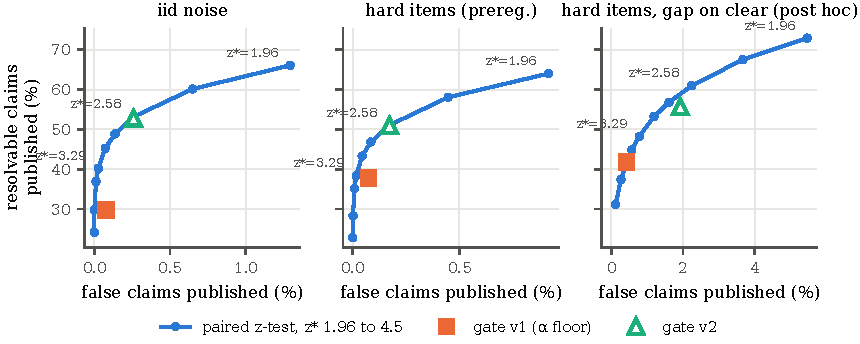
\includegraphics[width=\textwidth]{figures/gate_operating_points.pdf}
\caption{Share of false and resolvable claims published. Line: paired $z$-test with threshold 1.96 to 4.5. The third panel is a post-hoc scenario in which the better system's advantage lies on items the raters agree on.}
\label{fig:gate}
\end{figure*}

Gate~v1 published \simFalseVoneIid\% false and \simResVoneIid\% resolvable claims under independent noise; a $z$-test matched to its false-claim rate published \simResMatchedIid\% (Figure~\ref{fig:gate}). Part of the gap reflects the \simShareLowAlphaCells\% of cells with $\alpha<0.5$; restricted to $\alpha\geq0.5$ it narrows to \simResVoneIidHi\% vs.\ \simResMatchedIidHi\%. With errors concentrated on hard items the gap persists (\simResVoneHet\% vs.\ \simResMatchedHet\%), and only in a post-hoc scenario built to favour the floor do the two draw level (\simResVoneHetneg\% vs.\ \simResMatchedHetneg\%). Only the $\alpha$ floor and the MDE check ever bind; removing the floor raises the resolvable rate from \ablResNone\% to \ablResRel\% and the false-claim rate from \simFalseVoneIid\% to \ablFalseRel\%. Below $\alpha=0.5$ the floor blocks nearly every real difference (\simResVoneLowAlphaIid\% published, against \simResZlowLowAlphaIid\% for an ordinary test). Gate~v2's decisions are essentially a $z$-test at 2.58; its value is the report, whose attenuation estimate is on average within \attEstMaxErr of the truth at $n\geq1{,}000$.

\section{How reliable are real labels?}
\label{s:audit}
\begin{figure}[t]
\centering
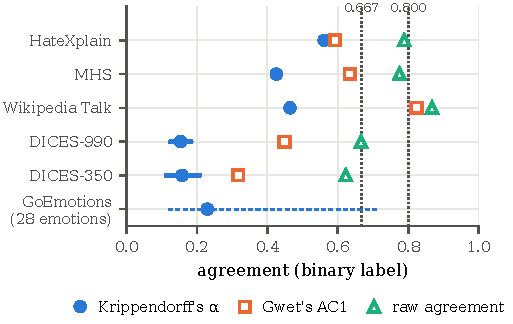
\includegraphics[width=\columnwidth]{figures/agreement.pdf}
\caption{Agreement on each corpus's binary label (95\% bootstrap intervals for $\alpha$).}
\label{fig:agree}
\end{figure}
We audit every corpus we found with rater identifiers and a research licence: HateXplain \citep{mathew2021hatexplain}, Measuring Hate Speech \citep{kennedy2020measuring}, Wikipedia Talk toxicity \citep{wulczyn2017ex}, DICES-350/990 \citep{aroyo2023dices} and GoEmotions \citep{demszky2020goemotions}. Main binary labels range from $\alpha=$ \alphaDthree to \alphaHx (Figure~\ref{fig:agree}); none reaches 0.667, and of GoEmotions' \nGoEmotions emotion labels only \goTopEmotion does. Coefficients diverge under skew: on Wikipedia Talk, $\alpha$ is \alphaWiki while AC1 is \acOneWiki. A threshold on one coefficient would pass or block the same labels depending on which coefficient was chosen.

\section{Could published gaps be resolved?}
\label{s:retro}
HateXplain's official test split has \retroN posts, \retroSplit\% of them 2--1 splits. Of the \retroPairs pairwise gaps between the six models in \citet[Table 6]{mathew2021hatexplain}, \retroUnresolvable (\retroMinGap to \retroBertGap) are significant at $z=1.96$ only if the two systems disagree on fewer than \retroMinPmax--\retroBertPmax\% of posts, including both comparisons that isolate rationale supervision. This is implausible even for two runs of one architecture. It concerns test size and accuracy only, not the paper's explainability claims; label noise would make it worse.

\section{LLM judges against a held-out human}
We scored five judges on up to 1,000 items per corpus against the panel majority, with one annotator held out and scored identically. On HateXplain, MHS and Wikipedia Talk no judge significantly exceeded the held-out human (best: \jSonnetHx vs.\ \jHumanHx, \jHaikuMhs vs.\ \jHumanMhs, \jSonnetWiki vs.\ \jHumanWiki). On DICES, where a single rater is a weak reference ($\alpha\approx$ \alphaDthree), three judges exceed the human (up to \jSonnetDthree vs.\ \jHumanDthree), yet on the dataset's expert labels four of five agree significantly less often than the crowd majority on the same items, and only Sonnet is indistinguishable from it (\exMDiffSonnet [\exMLoSonnet, \exMHiSonnet]); Sonnet's agreement drops to \jSonnetDthreeInvalidWrong if its \jSonnetDthreeUnparsed truncated outputs count as wrong. Gate~v2 resolved \jPairsPass of \jPairsTotal judge-versus-judge comparisons, none with a gap below 0.02; gate~v1 could publish \jPairsVonePub, all on HateXplain.

\section{Recommendations}
Report agreement with an interval and with AC1 and raw agreement beside $\alpha$; report the paired disagreement rate of compared systems; and report the smallest true gap the test size and label noise can resolve. Do not replace a significance test with a reliability threshold. At a fixed budget, label more items once rather than fewer items several times \citep{dorner2024dont}; in our real-rater test this held in all \clFourCells design cells.

\section*{Limitations}
The attenuation factor assumes binary labels, symmetric rater noise, and system errors independent of gold errors; we test departures with hard-item scenarios and real raters but cannot cover every structure. Two simulation scenarios were added after seeing results. The retrospective uses rounded published accuracies without system outputs and covers one paper. All corpora are English and five of six concern harmful content.

\section*{Ethics statement}
The corpora contain offensive text. We use them under their licences, quote no examples, and release only code, identifiers, labels and derived statistics. Stating that labels cannot resolve a gap is a statement about measurement, not a claim that any published result is wrong.

\ifdefined\PREPRINT\section*{Acknowledgements}\else\section*{Use of AI assistants}\fi
\ifdefined\PREPRINT This work received no external funding. \fi We used an AI coding assistant (Anthropic's Claude via Claude Code) to write and test analysis code, search for and verify related work, and draft text under the author's direction; the author checked the code and every citation and is responsible for the content.

\bibliography{references}
\end{document}
